\chapter{Argentinische Schaben (Dubia Roaches)}

\section{Säubern}
Gute Nachricht, das ist nicht nötig!

\section{Füttern}

\subsection{Trockenfutter}
Trockenfutter ist leicht anzubieten da es nicht schimmelt, einfach 1--2 Mal die Woche kontrollieren
und bei Bedarf die Futterschale auffüllen.
Trockenes Katzenfutter befindet sich im Gemüsefach des Kühlschranks, Haferflocken auf dem Tisch.
Nach Belieben entweder mischen oder einfach abwechseln.

\subsection{Frischfutter}
Gesund ernährte Schaben sind auch selbst gesünderes Futter, optional kann also gerne alle paar Tage
frisches Gemüse/Obst/Früchte gegeben werden. Sie freuen sich auch über Küchenreste.
Vorgeschnittenes Futter (Äpfel, Karotten, Pfirsich) liegt im oberen Fach des Tiefkühlers,
idealerwiese etwas antauen lassen bevor es den Schaben angeboten wird.

Von der Menge her nur so viel geben wie verzehrt wird, bevor es Schimmel ansetzt,
also z.B. 3--4 Karottenscheiben, ein Apfel-/Pfirsichstück oder ähnliches.
Lieber zu wenig geben als Schimmel riskieren.
Beim nächsten Besuch bitte kontrollieren und Reste entsorgen.

\section{Wasser}
Schaben ertrinken leicht, daher steht das Wasser in Form von Wasserperlen zur Verfügung.
Diese sollten nicht für mehr als einen Tag völlig austrocknen
(eine volle Schale Wasserperlen hält allerdings locker mehr als eine Woche),
daher lieber früher als später frische Perlen ansetzen:
\begin{enumerate}
  \item einen halben Teelöffel frische Perlen in Schale geben
  \item bis etwas über die Hälfte mit stillem Mineralwasser füllen
  \item abgedeckt einige Stunden (ggf. über Nacht) aufquellen lassen
  \item die ausgetrockneten Perlen in den bereitstehenden Becher umleeren
  \item frisch aufgequollene Perlen vorsichtig in die Wasserschale umfüllen\\
        (die Dinger springen wild umher)
\end{enumerate}
\begin{figure}[H]
  \begin{minipage}{.5\textwidth}
    \centering
    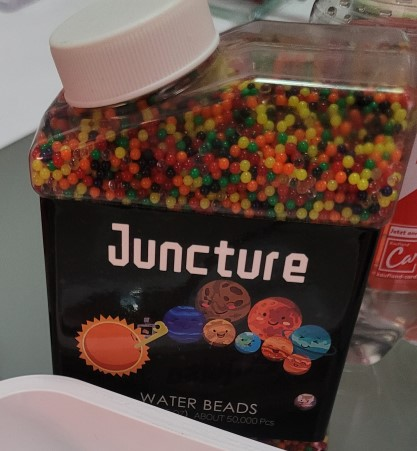
\includegraphics[width=.8\linewidth]{resources/Wasserperlen.jpg}
  \end{minipage}%
  \begin{minipage}{.5\textwidth}
    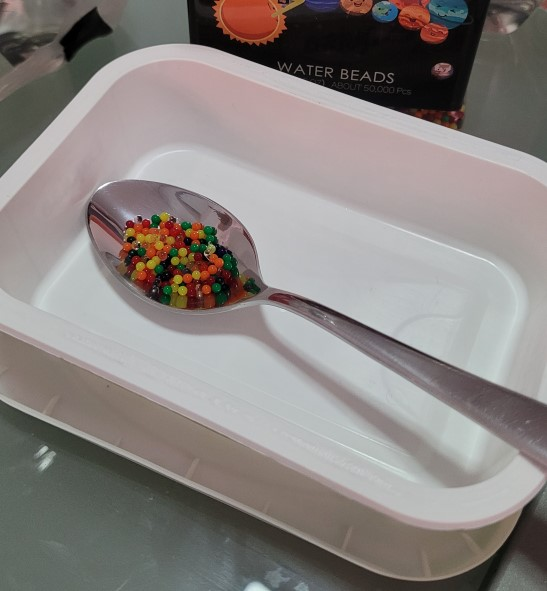
\includegraphics[width=.8\linewidth]{resources/Wasserperlen-abmessen.jpg}
  \end{minipage}
  \caption[Wasserperlen]{Menge an zu verwendender Perlen}
\end{figure}
